\subsection{Convection schemes}
\label{subsec:convection_schemes}

In this section, we will present the schemes related to the convection terms of the discretized governing equations, which were derived in Section \ref{subsec:application_of_the_finite_volume_method}.



%
% USD scheme
%
\subsubsection{\acrfull{uds}}

The \acrfull{uds} is the simplest convection scheme, and it is a $1^{th}-order$ scheme.

The idea behind the \acrshort{uds} is to consider the velocity at the face of the $U_{CV}$ equal to the upwind value between the current cell center value and the neighbor cell center value.

This means that \acrshort{uds} scheme can be visualized as:

\begin{figure}[H]
    \centering
    \begin{tikzpicture}

        \draw[->] (-0.5,0) -- (5,0) node[right] {$x$};
        \draw[->] (0,-1) -- (0,3) node[above] {$u(x)$};

        % \draw [blue, thick] plot [smooth] coordinates {(-0.5,1) (2.5,2) (4.5,-0.5)};

        \draw (0,0) node[below left] {$u_{WW}$} -- (0,1.22);
        \draw (0.5,0) node[below, shift={(0,-10pt)}] {$u_{ww}$} -- (0.5,0);
        \draw (1,0) node[below] {$u_W$} -- (1,1.68);
        \draw (1.5,0) node[below, shift={(0,-10pt)}] {$u_w$} -- (1.5,0);
        \draw (2,0) node[below] {$u_P$} -- (2,1.98);
        \draw (2.5,0) node[below, shift={(0,-10pt)}] {$u_e$} -- (2.5,0);
        \draw (3,0) node[below] {$u_E$} -- (3,1.62);
        \draw (3.5,0) node[below, shift={(0,-10pt)}] {$u_{ee}$} -- (3.5,0);
        \draw (4,0) node[below] {$u_{EE}$} -- (4,0.3);


        \filldraw[red] (0,1.22) circle (1pt);
        \filldraw[red] (1,1.68) circle (1pt);
        \filldraw[red] (2,1.98) circle (1pt);
        \filldraw[red] (3,1.62) circle (1pt);
        \filldraw[red] (4,0.3) circle (1pt);

        \draw [red] (0.5,1.68) -- (1,1.68);
        \draw [red] (1.5,1.98) -- (2,1.98);
        \draw [red] (2,1.98) -- (2.5,1.98);
        \draw [red] (3,1.62) -- (3.5,1.62);

        % Legend
        % \draw [blue] (5.5,2) -- (6,2) node[right] {Actual $\hat{u(x)}$};
        \draw [red] (5.5,1.5) -- (6,1.5) node[right] {Computed $u(x)$ using \acrshort{uds}};

    \end{tikzpicture}
    \caption{Example of the \acrshort{uds} scheme applied to the $u$ velocity component.}
    \label{fig:uds_convection_scheme}
\end{figure}

We can obtain a formula for the \acrshort{uds} that will be used in the implementation of the code.
In particular, by defining the Volume Fluxes as: $F_e = \hat{u_e} \Delta y$ \& $F_w = \hat{u_w} \Delta y$, we can write that:

\begin{align}
    u_e & = \begin{cases}
                u_P & \text{if } F_e > 0 \\
                u_E & \text{if } F_e < 0
            \end{cases} \\
    u_w & = \begin{cases}
                u_W & \text{if } F_w > 0 \\
                u_P & \text{if } F_w < 0
            \end{cases}
\end{align}

The same apply for the $v$ velocity component, but in this case, we will have $F_n = \hat{v_n} \Delta x$, $F_s = \hat{v_s} \Delta x$.

In the end, our \acrfull{uds} scheme applied to the convection term will be:

\begin{gather*}
    \left(\hat{u_e}u_e - \hat{u_w}u_w\right) \Delta y + \left(\hat{v_n}u_n - \hat{v_s}u_s\right) \Delta x = \\
    \left(F_e u_e - F_w u_w\right) + \left(F_n u_n - F_s u_s\right) = \\
    u_P*max(F_e, 0) + u_E*min(F_e, 0) + u_W*max(F_w, 0) + u_P*min(F_w, 0) + \\
    u_P*max(F_n, 0) + u_N*min(F_n, 0) + u_S*max(F_s, 0) + u_P*min(F_s, 0)
\end{gather*}

Since we are interested in the $A_P^\phi$ and $A_{nb}^\phi$ coefficients as written in the form of Equation \ref{eq:coefficients_form_system}, with the help of \texttt{Mathematica}, we can regroup the terms based on the velocity components, perform some sign manipulations and obtain the coefficients for the convection term using the \acrshort{uds} scheme for both the $u$ and $v$ momentum equations.

\begin{equation}
    \text{Convection Coefficients \acrshort{uds}:} = { \textbf{See table \ref{tab:Ap_coefficients}} }
\end{equation}



%
% CDS scheme
%
\subsubsection{\acrfull{cds}}

The \acrfull{cds} is a $2^{nd}-order$ scheme.

The idea behind the \acrshort{cds} is to consider the velocity at the face of the control volume as the average between the current cell center value and the neighbor cell center value.

This means that \acrshort{cds} scheme can be visualized as:

\begin{figure}[H]
    \centering
    \begin{tikzpicture}

        \draw[->] (-0.5,0) -- (5,0) node[right] {$x$};
        \draw[->] (0,-1) -- (0,3) node[above] {$u(x)$};

        % \draw [blue, thick] plot [smooth] coordinates {(-0.5,1) (2.5,2) (4.5,-0.5)};

        \draw (0,0) node[below left] {$u_{WW}$} -- (0,1.22);
        \draw (0.5,0) node[below, shift={(0,-10pt)}] {$u_{ww}$} -- (0.5,0);
        \draw (1,0) node[below] {$u_W$} -- (1,1.68);
        \draw (1.5,0) node[below, shift={(0,-10pt)}] {$u_w$} -- (1.5,0);
        \draw (2,0) node[below] {$u_P$} -- (2,1.98);
        \draw (2.5,0) node[below, shift={(0,-10pt)}] {$u_e$} -- (2.5,0);
        \draw (3,0) node[below] {$u_E$} -- (3,1.62);
        \draw (3.5,0) node[below, shift={(0,-10pt)}] {$u_{ee}$} -- (3.5,0);
        \draw (4,0) node[below] {$u_{EE}$} -- (4,0.3);


        \filldraw[red] (0,1.22) circle (1pt);
        \filldraw[red] (1,1.68) circle (1pt);
        \filldraw[red] (2,1.98) circle (1pt);
        \filldraw[red] (3,1.62) circle (1pt);
        \filldraw[red] (4,0.3) circle (1pt);

        \draw [red] (0,1.22) -- (1,1.68);
        \draw [red] (1,1.68) -- (2,1.98);
        \draw [red] (2,1.98) -- (3,1.62);
        \draw [red] (3,1.62) -- (4,0.3);

        % Legend
        % \draw [blue] (5.5,2) -- (6,2) node[right] {Actual $\hat{u(x)}$};
        \draw [red] (5.5,1.5) -- (6,1.5) node[right] {Computed $u(x)$ using \acrshort{cds}};

    \end{tikzpicture}
    \caption{Example of the \acrshort{cds} scheme applied to the $u$ velocity component.}
    \label{fig:cds_convection_scheme}
\end{figure}

We can obtain a formula for the \acrshort{cds} that will be used in the implementation of the code.
In particular, by using the same definition of the Volume Fluxes as before, we can write that:

\begin{align}
    u_e & = \frac{u_P + u_E}{2} \\
    u_w & = \frac{u_W + u_P}{2}
\end{align}

The same apply for the $v$ velocity component.

In the end, our \acrshort{cds} scheme applied to the convection term will be:

\begin{gather*}
    \left(\hat{u_e}u_e - \hat{u_w}u_w\right) \Delta y + \left(\hat{v_n}u_n - \hat{v_s}u_s\right) \Delta x = \\
    \left(F_e u_e - F_w u_w\right) + \left(F_n u_n - F_s u_s\right) = \\
    F_e \frac{u_P + u_E}{2} - F_w \frac{u_W + u_P}{2} + F_n \frac{u_P + u_N}{2} - F_s \frac{u_S + u_P}{2}
\end{gather*}

Since we are interested in the $A_P^\phi$ and $A_{nb}^\phi$ coefficients as written in the form of Equation \ref{eq:coefficients_form_system}, with the help of \texttt{Mathematica}, we can regroup the terms based on the velocity components, perform some sign manipulations and obtain the coefficients for the convection term using the \acrshort{cds} scheme for both the $u$ and $v$ momentum equations.

\begin{equation*}
    \text{Convection Coefficients \acrshort{cds}:} = { \textbf{See table \ref{tab:Ap_coefficients}} }
\end{equation*}



%
% QUICK scheme
%
\subsubsection{\acrfull{quick}}

The \acrfull{quick} is a $3^{rd}-order$ scheme.

The idea behind the \acrshort{quick} scheme is to interpolate the velocity at the center of 3 cells to then compute the velocity at the face of the cell.
The choice of the cells to interpolate is based on the direction of the velocity at previous step ($\hat{u}$ or $\hat{v}$) similarly to the \acrshort{uds} scheme.
For example, if we are computing the $u_e$ velocity, we will pick as interpolations points the $u_P$, $u_E$ velocity and $u_{EE}$ or $u_{W}$ based on the direction of the velocity at the face.

The \acrshort{quick} scheme can be visualized as:

\begin{figure}[H]
    \centering
    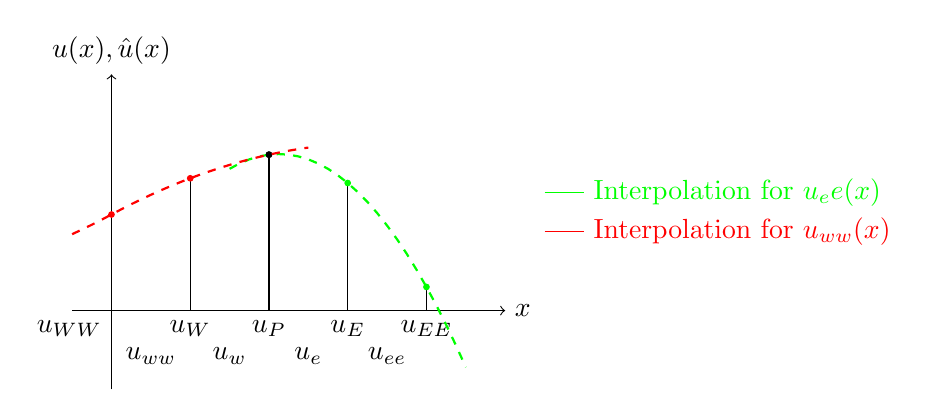
\begin{tikzpicture}

        \draw[->] (-0.5,0) -- (5,0) node[right] {$x$};
        \draw[->] (0,-1) -- (0,3) node[above] {$u(x), \hat{u}(x)$};

        % \draw [blue, thick] plot [smooth] coordinates {(-0.5,1) (2.5,2) (4.5,-0.5)};

        \draw (0,0) node[below left] {$u_{WW}$} -- (0,1.22);
        \draw (0.5,0) node[below, shift={(0,-10pt)}] {$u_{ww}$} -- (0.5,0);
        \draw (1,0) node[below] {$u_W$} -- (1,1.68);
        \draw (1.5,0) node[below, shift={(0,-10pt)}] {$u_w$} -- (1.5,0);
        \draw (2,0) node[below] {$u_P$} -- (2,1.98);
        \draw (2.5,0) node[below, shift={(0,-10pt)}] {$u_e$} -- (2.5,0);
        \draw (3,0) node[below] {$u_E$} -- (3,1.62);
        \draw (3.5,0) node[below, shift={(0,-10pt)}] {$u_{ee}$} -- (3.5,0);
        \draw (4,0) node[below] {$u_{EE}$} -- (4,0.3);

        % u_ee interpolation
        \filldraw[black] (2,1.98) circle (1pt);
        \filldraw[green] (3,1.62) circle (1pt);
        \filldraw[green] (4,0.3) circle (1pt);
        \draw [green, thick, dashed] plot[domain=1.5:4.5] (\x, {-0.48*\x^2 + 2.04*\x - 0.18});

        % w_ww interpolation
        \filldraw[red] (0,1.22) circle (1pt);
        \filldraw[red] (1,1.68) circle (1pt);
        \filldraw[black] (2,1.98) circle (1pt);
        \draw [red, thick, dashed] plot[domain=-0.5:2.5] (\x, {-0.08*\x^2 + 0.54*\x + 1.22});

        % Legend
        % \draw [blue] (5.5,2) -- (6,2) node[right] {Actual $\hat{u}(x)$};
        \draw [green] (5.5,1.5) -- (6,1.5) node[right] {Interpolation for $u_ee(x)$};
        \draw [red] (5.5,1) -- (6,1) node[right] {Interpolation for $u_{ww}(x)$};

    \end{tikzpicture}
    \caption{Example of the \acrshort{quick} scheme applied to the $u$ velocity component.}
    \label{fig:quick_convection_scheme}
\end{figure}

We can obtain a formula for the \acrshort{quick} that will be used in the implementation of the code.
In particular, we can recall the definition of the Lagrange interpolation polynomial of degree 2:

\begin{equation}
    P(x) = \sum_{i=0}^{2} y_i \prod_{j=0, j \neq i}^{2} \frac{x - x_j}{x_i - x_j}
    \label{eq:langrange_interpolation_polynomial}
\end{equation}

In our case, it's convenient to fix the reference system in correspondence of the center of the control volume considered.
If that is the case, then for example the evaluation of the velocity at the face $u_e$ will be:

\begin{equation}
    u_e = P(x) \bigg|_{x = \Delta x/2}
\end{equation}

As we said before, the choice of the interpolation points is based on the direction of the velocity at the face of the control volume.
In particular, if we are computing the $u_e$ velocity, the possible polynomials ($P_e(x)$) will be:

\begin{equation}
    P_e(x) = \begin{cases}
        P(u_W, u_P, u_E)    & \text{if } \hat{u_e} > 0 \\
        P(u_P, u_E, u_{EE}) & \text{if } \hat{u_e} < 0
    \end{cases}
\end{equation}

By using \texttt{Mathematica}, we can compute the polynomials for the $u$ velocity component in both cases.

The results of the symbolic analysis are:

\begin{align}
    u_e & = \begin{cases}
                -\frac{1}{8} u_W + \frac{3}{4} u_P + \frac{3}{8} u_E    & \text{if } \hat{u_e} > 0 \\
                +\frac{3}{8} u_P + \frac{3}{4} u_E - \frac{1}{8} u_{EE} & \text{if } \hat{u_e} < 0
            \end{cases}    \\
    u_w & = \begin{cases}
                -\frac{1}{8} u_{WW} +    \frac{3}{4} u_W + \frac{3}{8} u_P & \text{if } \hat{u_w} > 0 \\
                +\frac{3}{8} u_W + \frac{3}{4} u_P - \frac{1}{8} u_E       & \text{if } \hat{u_w} < 0
            \end{cases}
\end{align}

The same apply for the $v$ velocity component, but in this case, the variables that decide the interpolation points are the $\hat{v_n}$ and $\hat{v_s}$.

In the end, our \acrshort{quick} scheme applied to the convection term will be:

\begin{gather}
    \left(\hat{u_e}u_e - \hat{u_w}u_w\right) \Delta y + \left(\hat{v_n}u_n - \hat{v_s}u_s\right) \Delta x = \\
    \left(F_e u_e - F_w u_w\right) + \left(F_n u_n - F_s u_s\right) = \\
    \frac{1}{8} (
    (3 u_{E} + 6 u_{P} - u_{W}) max(0, F_e) + (- u_{EE} + 6 u_{E} + 3 u_{P}) min(0, F_e) + \\
    (- 3 u_{P} - 6 u_{W} + u_{WW}) max(0, F_w) + (u_{E} - 6 u_{P} - 3 u_{W}) min(0, F_w) + \\
    (3 u_{N} + 6 u_{P} - u_{S}) max(0, F_n) + (6 u_{N} - u_{NN} + 3 u_{P}) min(0, F_n) + \\
    (- 3 u_{P} - 6 u_{S} + u_{SS}) max(0, F_s) + (u_{N} - 6 u_{P} - 3 u_{S}) min(0, F_s)
    )
\end{gather}

Since we are interested in the $A_P^\phi$ and $A_{nb}^\phi$ coefficients as written in the form of Equation \ref{eq:coefficients_form_system}, with the help of \texttt{Mathematica}, we can regroup the terms based on the velocity components, perform some sign manipulations and obtain the coefficients for the convection term using the \acrshort{quick} scheme for both the $u$ and $v$ momentum equations.

\begin{equation*}
    \text{Convection Coefficients \acrshort{quick}:} = { \textbf{See table \ref{tab:Ap_coefficients}} }
\end{equation*}



% %
% % Hybrid scheme
% %
% \subsubsection{\acrfull{hybrid}}

% The \acrfull{hybrid} combines the \acrshort{uds} and \acrshort{cds} schemes based on the Peclet number $P_e$.

% The Peclet number can be defined at each face of the control volume as:

% \begin{align}
%     Pe_e & = \frac{\hat{u_e} \Delta x}{\nu} \\
%     Pe_w & = \frac{\hat{u_w} \Delta x}{\nu} \\
%     Pe_n & = \frac{\hat{v_n} \Delta y}{\nu} \\
%     Pe_s & = \frac{\hat{v_s} \Delta y}{\nu}
% \end{align}

% By doing so, we can now define the \acrshort{hybrid} scheme as:

% \begin{equation}
%     \text{Convection Coefficients \acrshort{hybrid}:} = \begin{cases}
%         \text{UDS} & \text{if } Pe > 2 \\
%         \text{CDS} & \text{if } Pe < 0.5
%     \end{cases}
% \end{equation}


